%  !TeX  root  =  user_guide.tex

\section{Модуль экспорта в файл проекта MapServer}\label{sec:mapserver_export}

% when the revision of a section has been finalized,
% comment out the following line:
%\updatedisclaimer

Существует возможность использования QGIS для <<создания>> карты для MapServer
путем добавления и распределения слоев, нанесения обозначений и определения цветов.

\subsection{Создание файла проекта}

Модуль экспорта в MapServer оперирует с сохраненным проектом QGIS, а
\textbf{не} с текущим содержимым окна с картой и легендой слоев. У
многих пользователей это вызвало значительное замешательство. Как
описано ниже, перед тем, как использовать модуль экспорта, требуется
предварительное распределение растровых и векторных слоев, которые нужно
использовать в MapServer, и последующее сохранение в файле проекта QGIS.

\begin{figure}[ht]
\centering
  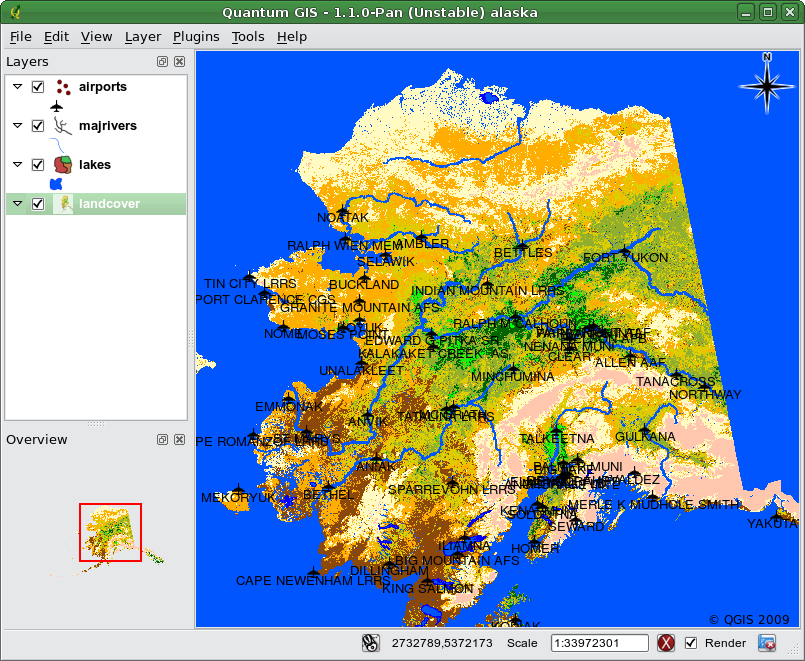
\includegraphics[clip=true, width=12cm]{mapserver_export_qgis}
   \caption{Распределение растровых и векторых слоев для проекта QGIS \wincaption}
  \label{fig:mapserver_export_qgs}
\end{figure}

В этом примере будут продемонстрированы четыре этапа, необходимых для
создания простого проекта, из которого получится карта
для MapServer. Будут использованы растровые и векторные файлы из
пробного набора QGIS \ref{label_sampledata}.

\begin{enumerate}
\item Добавьте растровый слой \filename{landcover.tif}, нажав на иконку
\toolbtntwo{mActionAddRasterLayer}{Добавить растровый слой}.
\item Добавьте векторные shape-файлы \filename{lakes.shp, majrivers.shp}
и \filename{airports.shp} из пробного набора QGIS, нажав на иконку
\toolbtntwo{mActionAddNonDbLayer}{Добавить векторный слой}.
\item Измените цвета и вид представления данных по вашему усмотрению
(к примеру, см. Рисунок~\ref{fig:mapserver_export_qgs})
\item Сохраните новый проект под названием \filename{mapserverproject.qgs}
следующим путем: \\
\mainmenuopt{Файл} \arrow \dropmenuopttwo{mActionFileSave}{Сохранить проект}.
\end{enumerate}

\subsection{Создание карты}

Инструмент \filename{msexport}, применяемый для экспорта проекта QGIS
в файл карты MapServer, установлен в каталог бинарных файлов QGIS и
может использоваться независимо от QGIS. Чтобы воспользоваться им из
QGIS, нужно сначала активировать модуль экспорта в MapServer через
<<Управление модулями>> (см. Раздел~\ref{sec:load_core_plugin}).

\begin{figure}[ht]
\centering
  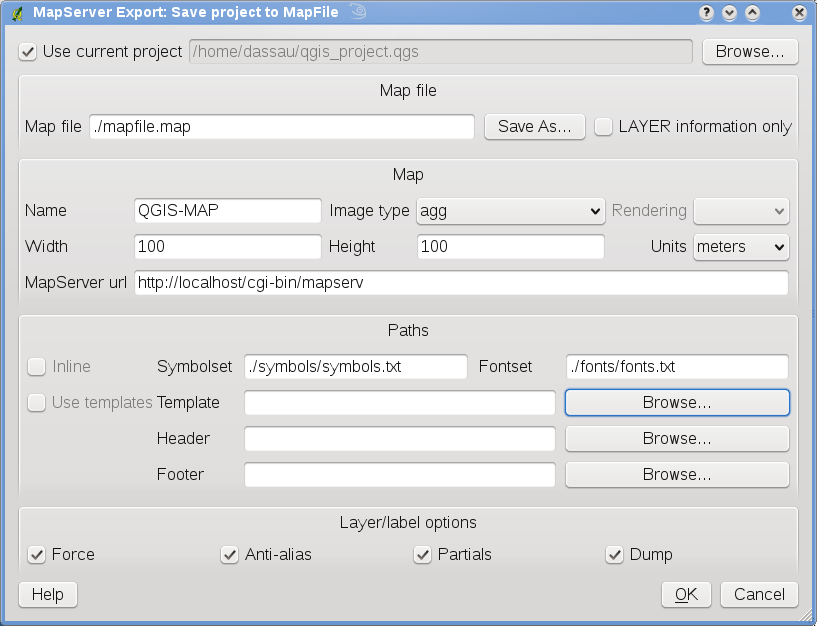
\includegraphics[clip=true, width=9cm]{mapserver_export_dialog}
  \caption{Диалоговое окно модуля экспорта в MapServer \wincaption}
  \label{fig:mapserver_export_dialog}
\end{figure}

\begin{description}
\item [Файл карты] \mbox{}\\
Введите название для создаваемого map-файла. Можно воспользоваться
кнопкой справа для перехода в директорию, где требуется сохранить файл
карты.
\item [Файл проекта Qgis] \mbox{}\\
Введите полный путь к экспортируемому файлу проекта QGIS (.qgs). Можно
воспользоваться кнопкой слева для перехода к файлу проекта QGIS.
\item [Имя карты] \mbox{}\\
Название карты. Это название будет ставиться в начало названий всех
изображений, созданных в mapserver.
\item [Ширина карты] \mbox{}\\
Ширина выходного изображения в пикселах.
\item [Высота карты] \mbox{}\\
Высота выходного изображения в пикселах.
\item [Единицы карты] \mbox{}\\
Единицы измерения, используемые для выходного изображения.
\item [Формат изображения] \mbox{}\\
Формат выходного изображения, созданного в MapServer.
\item [Шаблон] \mbox{}\\
Полный путь к файлу шаблона MapServer, применяемого к map-файлу.
\item [Верхний колонтитул] \mbox{}\\
Полный путь к файлу верхнего колонтитула MapServer, используемому с
map-файлом.
\item [Нижний колонтитул] \mbox{}\\
Полный путь к файлу нижнего колонтитула MapServer, используемому с
map-файлом.
\end{description}

Для создания map-файла необходимы лишь \filename{Файл карты} и
\filename{Файл проекта QGIS}, тем не менее, опуская другие параметры,
можно получить нефункциональный map-файл. Хотя QGIS отлично создает map-файлы из
предоставленных проектов, вполне возможно, что понадобится некоторая
настройка для получения нужных результатов. К примеру, мы создали
map-файл, использовав файл проекта \filename{mapserverproject.qgs},
который только что создали (см. Рисунок~\ref{fig:mapserver_export_dialog}):

\begin{enumerate}
  \item После нажатия на иконку \toolbtntwo{mapserver_export}{Экспорт в MapServer}
  на панели инструментов, запустится диалогое окно (см. Рисунок~\ref{fig:mapserver_export_dialog}).
  \item Введите название (например, \filename{qgisproject.map}) для
  нового map-файла.
  \item Перейдите и найдите файл проекта QGIS
  (например, \filename{mapserverproject.qgs}), который перед этим
  сохранили.
  \item Введите название (к примеру, \filename{MyMap}).
  \item Введите ширину и высоту (к примеру, \filename{600} в качестве
  ширины и \filename{400}~--- высоты) для результирующего изображения.
  \item В данном примере слои измеряются в метрах, потому единицы
  измерения выставляются в метрах.
  \item Выберите <<png>> в качестве формата изображения.
  \item Нажмите кнопку \button{OK} для того, чтобы создать новый
  map-файл \filename{qgisproject.map}. QGIS выведет сообщение об
  удачном завершении операции.
\end{enumerate}

Map-файл можно просмотреть в любом тектовом редакторе или просмотрщике.
Если присмотреться, то можно заметить, что инструмент экспортирования
добавляет метаданные, нужные для того, чтобы map-файл мог быть
задействован в WMS (Web Map Service).

\subsection{Проверка map-файла}

Теперь можно протестировать результат проделанного, использовав
инструмент \filename{shp2img} для создания изображения из map-файла.
Утилита \filename{shp2img} является частью MapServer и набора
инструментов FWTools. Для
создания изображения из нашей карты необходимо:

\begin{itemize}[label=--]
\item Открыть окно консоли
\item Если map-файл не был сохранен в домашнем каталоге, перейти в
директорию, куда он был сохранен.
\item Запустить \filename{shp2img -m qgisproject.map -o mapserver\_test.png}
и открыть изображение.
\end{itemize}

Будет создан файл PNG, включающий все слои, содержащиеся в файле проекта
QGIS. Кроме того, охват файла PNG останется таким же, как и когда
проект был сохранен. Как можно увидеть на
рисунке~\ref{fig:mapserver_export_test}, вся информация за исключением
обозначений аэропортов включена.

\begin{figure}[ht]
\centering
  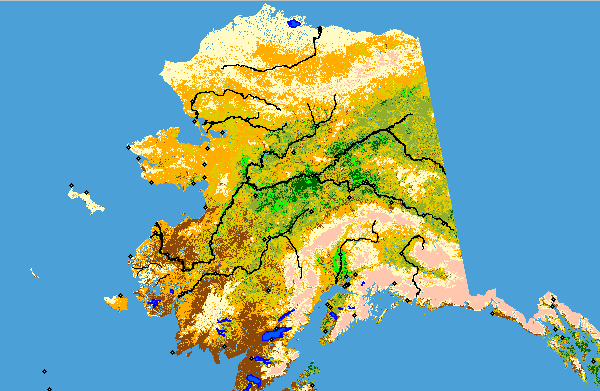
\includegraphics[clip=true, width=10cm]{mapserver_export_test}
  \caption{Тестовый файл PNG, созданный с помощью shp2img со всеми экспортированными слоями \wincaption}
  \label{fig:mapserver_export_test}
\end{figure}

Если планируется использовать map-файл для обработки запросов WMS,
скорее всего, не нужно что-либо перенастраивать. Если же планируется
использовать его в качестве карты-шаблона или специализированного
интерфейса, возможно, понадобится проделать некоторую ручную работу.
Чтобы увидеть, насколько быстр переход от QGIS к обработке карт в Сети,
рекомендуем посмотреть 5-минутное онлайн-видео от Кристофера Шмидта. Он
использовал более старую версию QGIS (0.8), но видео в равной
степени отображает функции, присущие новым версиям.
\footnote{\url{http://openlayers.org/presentations/mappingyourdata/}}

\FloatBarrier
